\documentclass{sig-alternate-05-2015}

\makeatletter
\def\@copyrightspace{\relax}
\makeatother

\usepackage{verbatim}
\usepackage{graphicx}
\usepackage{gensymb}

\begin{document}

\title{CS701 Final Project Report}
%\subtitle{}

\numberofauthors{2} % 2 authors in this file

\author{
% You can add or remove blocks as needed.
%
% 1st. author
\alignauthor
Leo McElroy\\
       \affaddr{Middlebury College}\\
       \affaddr{Middlebury, VT}\\
       \email{lmcelroy@middlebury.edu}
% 2nd. author
\alignauthor
Ben Brown\\
       \affaddr{Middlebury College}\\
       \affaddr{Middlebury, VT}\\
       \email{bwbrown@middlebury.edu}
}

\maketitle

\begin{abstract}

	Prepare a 1-2 paragraph abstract that summarizes the project objective,
	motivation, and a brief description of your final results and conclusions.
	The abstract should be approximately 300-500 words.

\end{abstract}


\keywords{CS701; \LaTeX;}



\section{Introduction}


%State your problem and provide the motivation for solving/studying it: Why is
%the problem important? In which field of computer science does it fit?  What
%novel contribution does your project make? Your introduction should end with a
%brief outline for the organization of the rest of the paper. This section
%should be approximately 1 page in length.

In the the last ten years the popularization of 3D printers and makerspaces has caused interest in digital fabricators to blossom. Digital fabricators are machines which use computer controlled tools to produce 3D objects. The digital fabrication workflow begins in a computer-aided design (CAD) program where the user produces electronic schematics. These schematics are then brought into a computer-aided manufacturing (CAM) program where the user creates tool paths for a computer numerical control (CNC) machine, this process outputs instructions for the fabrication machine. Finally these instructions are uploaded to a digital fabricator and the schematic is recreated in the medium worked by the fabrication machine. Depending on the machine this medium can be plastic, paper, cardboard, metal, stone, wood, glass, or even organic material. The digital fabrication workflow is depicted in Figure \ref{fig:digiFabWorkflow}.

\begin{figure}[H]
  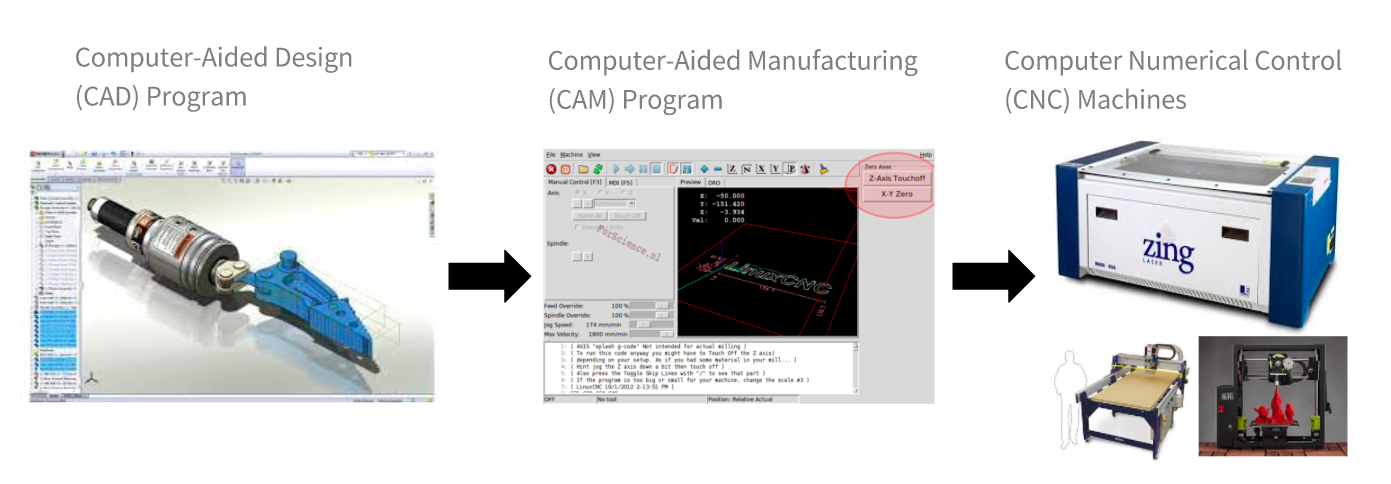
\includegraphics[width=\linewidth]{digiFabWorkflow.jpg}
  \caption{The digital fabrication workflow from CAD to CAM to digital fabricator.}
  \label{fig:digiFabWorkflow}
\end{figure}

Personal digital fabricators, or fabricators intended for use outside of an industrial manufacturing setting (think personal computer versus mainframe), include 3D printers, computer-numerical-control (CNC) mills, and laser cutters. Laser cutters are often considered the best balance of accessibility and usefulness of these digital fabricators. A laser cutter works by focusing a high powered laser through a focusing head which is attached to a gantry. The gantry controls the position of the head and therefore the location of the laser on a workpiece that rests on a bed underneath the gantry. A top-view schematic of a laser cutter is depicted in Figure~\ref{fig:lasersystem}.

\begin{figure}[H]
  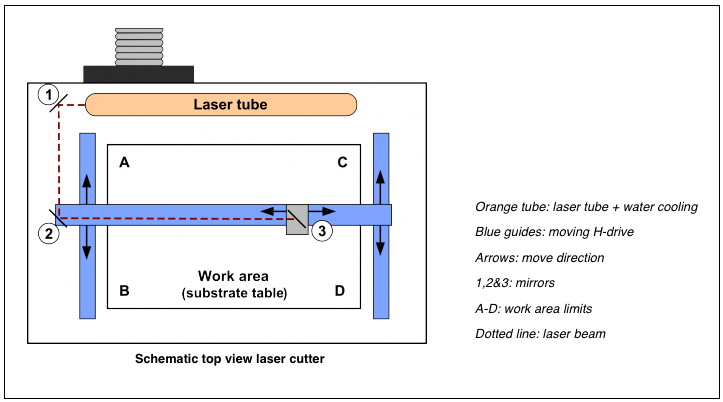
\includegraphics[width=\linewidth]{lasersystem.jpg}
  \caption{Top-view schematic of laser cutter adapted from Ref. \cite{laos}.}
  \label{fig:lasersystem}
\end{figure}

Laser cutters are capable of cutting and engraving. Most commercial laser cutters will cut plastic, paper, cardboard, and wood up to a quarter inch thick. They can also engrave all these materials and most types of metal and glass.

There are two main paradigms for modeling in CAD programs - direct modeling and parametric modeling. In direct modeling the user interacts directly with the geometry. This is typically through transformations such as dragging, rotating, or scaling. In parametric modeling the design program utilizes a geometric constraint solver that allows the user to specify constraints and dimensions on geometry. The design is then automatically adjusted to satisfy these constraints when the user modifies geometry directly. Figure~\ref{fig:parametricProgram} depicts the common constraint capabilities of a parametric design program.

\begin{figure}[H]
  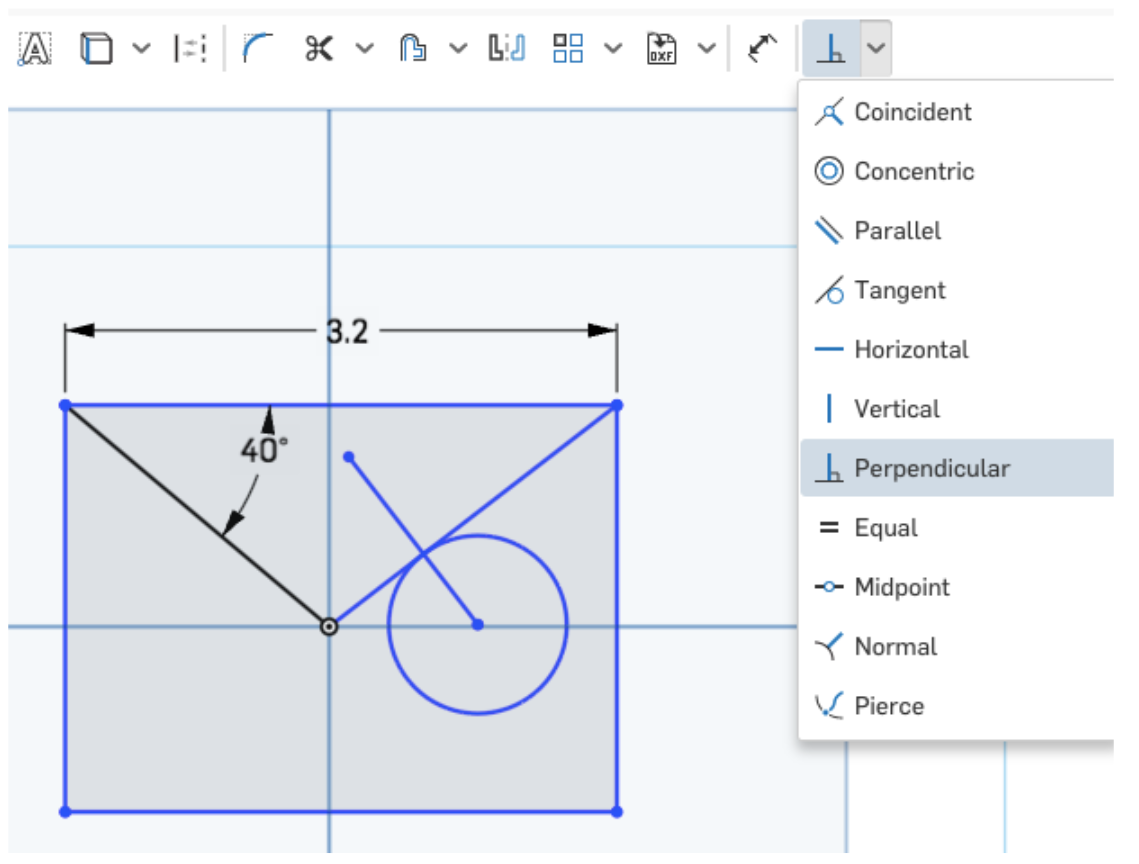
\includegraphics[width=\linewidth]{parametricProgram.jpg}
  \caption{Screenshot of parametric CAD program (Onshape) which shows common geometric constraints.}
  \label{fig:parametricProgram}
\end{figure}

Laser cutters are typically 2-dimensional fabricators which means there is no $z$-axis adjustability during fabrication. Consequently, prevalent drawing programs such as Adobe Illustrator and CorelDRAW were adopted for creating designs intended for laser cutting. Vector graphics, a scale-agnostic format where images are represented mathematically, are typically used for generating cutting paths. Rasters, a format where images are represented by pixels, are typically interpreted as engravings when laser cutting.

The issue that motivated our project is that the laser cutting workflow is often made unnecessarily cumbersome by users switching between various design programs. These include parametric CAD programs, with features intended for designing 3D real objects, and high-powered drawing programs, with features intended for creating intricate drawings. Our project aims to unify the essential features for laser cutting found in each of these design softwares into one program.

In Section 2 we present the current issue with the laser cutting workflow and design process. In Section 3 we briefly review programs with some of the features we were interested in incorporating into 2to3D. In Section 4 we describe the basic shape tools and how we handle geometric constraints using Cassowary.js. In Section 5 we cover the rest of functionality and capabilities of the 2to3D program. And in Section 6 we discuss the success of the project, review the major design principal of 2to3D, and describe extensions to our work which will result in 2to3D becoming a viable substitute for existing programs used for laser cutting. 

\section{Problem Statement}

The problem we attempted to solve is that existing CAD programs are not designed for laser cutting. Laser cutting requires 2D schematics so non-parametric drawing programs are appealing to use but laser cutters produce 3D objects so parametric design capabilities are highly desirable. Parametric design is based on setting constraints and dimensions (the way an engineer would design). This approach facilitates creating real objects. The need for parametric design and basic drawing capabilities results in users switching between a variety of programs which each offer some subset of desired features. Consequently users often find themselves switching back and forth between programs when creating designs. This issue with the current laser cutting workflow is depicted in Figure~\ref{fig:laserCuttingWorkflow}. A user creates the skeleton for a design in a parametric CAD program intended for modeling 3D objects (such as Onshape, Fusion360, or Solidworks). The user then imports this design into a some vector drawing software (Adobe Illustrator or CorelDRAW), then into a program capable of producing tool-paths (in this case CorelDRAW), which are finally sent to the laser cutter.

\begin{figure}[!h]
  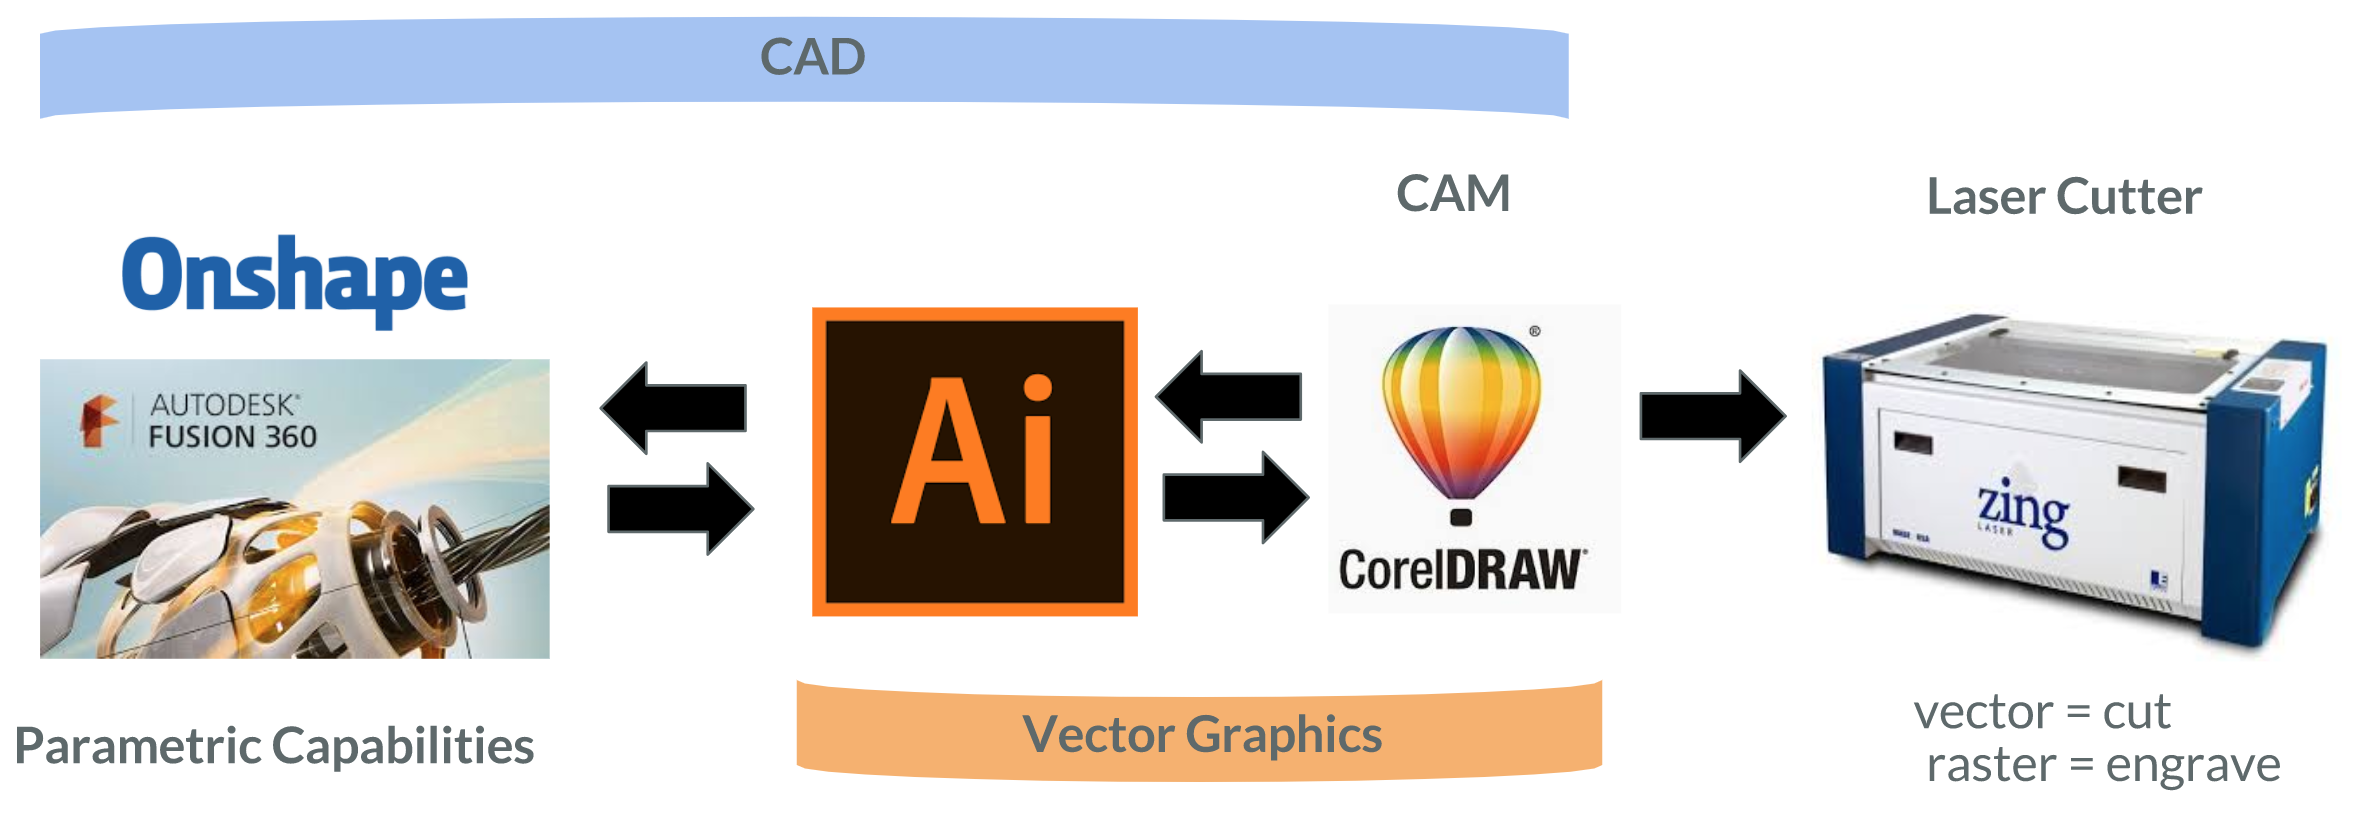
\includegraphics[width=\linewidth]{laserCuttingWorkflow.jpg}
  \caption{The current laser cutting workflow. Notice the ``pong effect" between design programs in the CAD portion of the workflow.}
  \label{fig:laserCuttingWorkflow}
\end{figure}


Another issue with the current laser cutting workflow is the price and complexity of commercial CAD software. Be it parametric CAD - Onshape, Fusion360, Solidworks - or visual design software - the Adobe Suite, CorelDRAW - commercial design software often requires a user pay regular subscription fees or retains ownership over user produced data. This makes laser cutting inaccessible to new hobbyists who may be unwilling to pay the fees or concerned with privacy of files they create. Additionally existing CAD software is over-engineered and inappropriate for a majority laser cutting tasks. most parametric CAD programs also incorporate sculpting and constructive solid geometry (CSG) tools which are completely irrelevant to a user interested in laser cutting. Likewise visual design programs involve complex layering systems and style modification tools with no relevance to physical designs. An ideal CAD program for laser cutting would incorporate features of both traditional drawing programs and parametric design programs. Our goal was to create a single-page web-based program specifically designed for laser cutting. A program that combined the best parts of 2D drawing programs and 3D CAD programs, while leaving the unnecessary parts behind. Specifically, we wanted our program to be SVG based so that drawings could be easily sent to a laser cutter, and we wanted to incorporate a geometric constraint solver so that we could easily create real-world objects. The laser cutting workflow we would ultimately want to create would involve one program for producing all designs and tool paths. This is depicted in Figure~\ref{fig:2to3DWorkflow}.

\begin{figure}[h]
  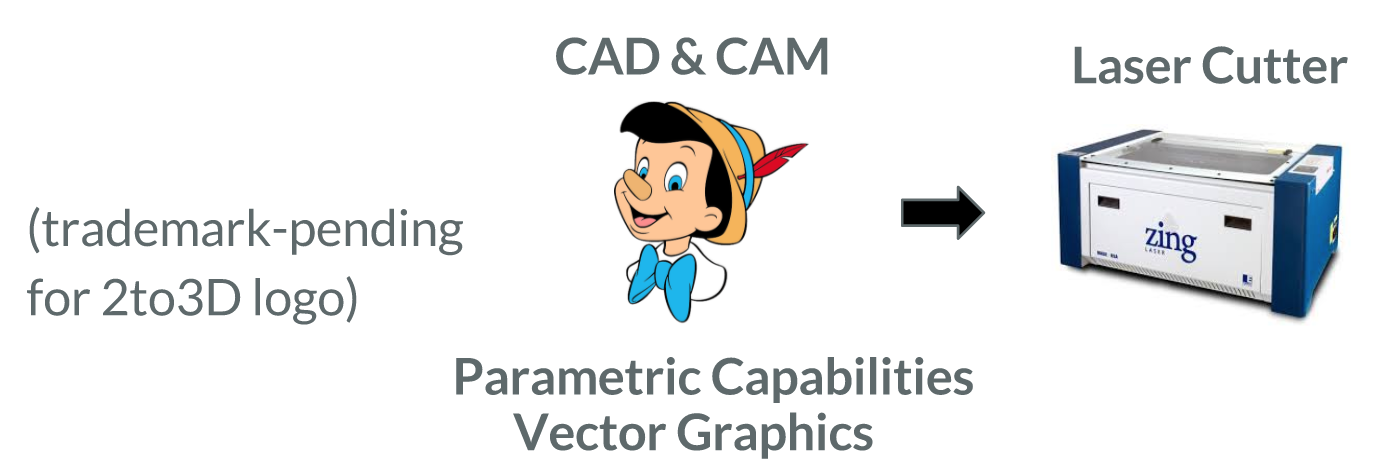
\includegraphics[width=\linewidth]{2to3DWorkflow.jpg}
  \caption{The laser cutting workflow we aim to create.}
  \label{fig:2to3DWorkflow}
\end{figure}

Semester time constraints meant we did not incorporate CAM or engraving features into 2to3D.


\section{Related Work}

%Provide a review of prior work that is similar to yours. Who else has
%solved/researched this problem or similar problems? What was their approach?
%How is your research new and different? Here you can describe shortcomings in
%previous work that your work complements and or improves upon. This section
%should be approximately 0.5-1 page in length depending on the amount of related
%work.

\begin{itemize}
  \item \textbf{Easel from Inventables}: Easel is a web-based CAD program for CNC (computer numerical control) milling. It is non-parametric and integrated with CAM (computer aided manufacturing), this means it is capable of outputting G-Code.
  \item \textbf{Vectr}: Vectr is a simple vector drawing program capable of running in the browser. The drawing features are very similar to what we plan to implement.
  \item \textbf{Onshape}: Onshape is a commercial 3D parametric CAD program which is also web-based and integrated with CAM.
  \item \textbf{SolveSpace}:
  \item \textbf{jSketcher}: 
\end{itemize}


\section{Methods}

There were two main parts of 2to3D we needed to implement: the user interface and the geometric constraint solver. For each of these tasks, we employed a different library, with lots of JavaScript code gluing them together.

\subsection*{User Interface with React.js}

React.js is an innovative JavaScript library that allows the programmer to specify different parts of the interface as {\it components}. Each component manages its own state and has its own render function. Whenever a component's state is changed, React automatically re-renders it, effectively abstracting the render loop from the programmer. In this way, a typical React App need only deal with event handling by manipulating state.

2to3D consists of one main DrawArea component, whose state contains all the primitive shape objects, along with the constraints on these objects, so that when the user draws a new shape or modifies an existing one, the interface is re-rendered.

%The state of each object consists of where it is located in the drawing region and whether or not the shape is selected. Furthermore, each shape maintains its own render method, which is based on the aforementioned aspects of state.

Currently, we have the following shape primitives:

\begin{itemize}
\item {\bf Freehand Curves}
\item {\bf Lines}
\item {\bf Bezier Curves}
\end{itemize}

Freehand curves are simply SVG paths, but within Line and Bezier objects are points whose values can be manipulated, both by the user and the constraint solver. We discuss this in more detail in the next section, but with these shape primitives we created the following drawing tools:

\begin{itemize}
\item {\bf Freehand:} Simply draws a freehand curve following the cursor.
\item {\bf Polyline:} Creates lines where adjacent endpoints are constrained to be coincident, optionally allowing the user to close the polyline where it started, creating a polygon.
\item {\bf Bezier:} Creates bezier curves whose adjacent endpoints are constrained to be coincident and adjacent control points are constrained to be collinear with the endpoint between them.
\item {\bf Rectangle:} Creates four lines in a rectangle where the top and bottom lines are constrained to be horizontal and the left and right lines are constrained to be vertical.
\end{itemize}

\subsection*{Geometric Constraints with Cassowary.js}

In order to design physical objects for laser cutting, we needed our program to implement geometric constraints. For example, we would like to be able to specify two lines as parallel, or a line have fixed length. All of the constraints we wanted to implement can be represented as systems of equations. For example, consider Figure \ref{fig:constraints} below. We constrain point $a$ to always lie on the circle of radius 1, we fix the line with endpoints $a$ and $b$ to have length $\sqrt{2}$ using the distance equation, and we set the line with endpoints $b$ and $c$ to lie on the $x$-axis and have length 1.

\begin{figure}[H]
  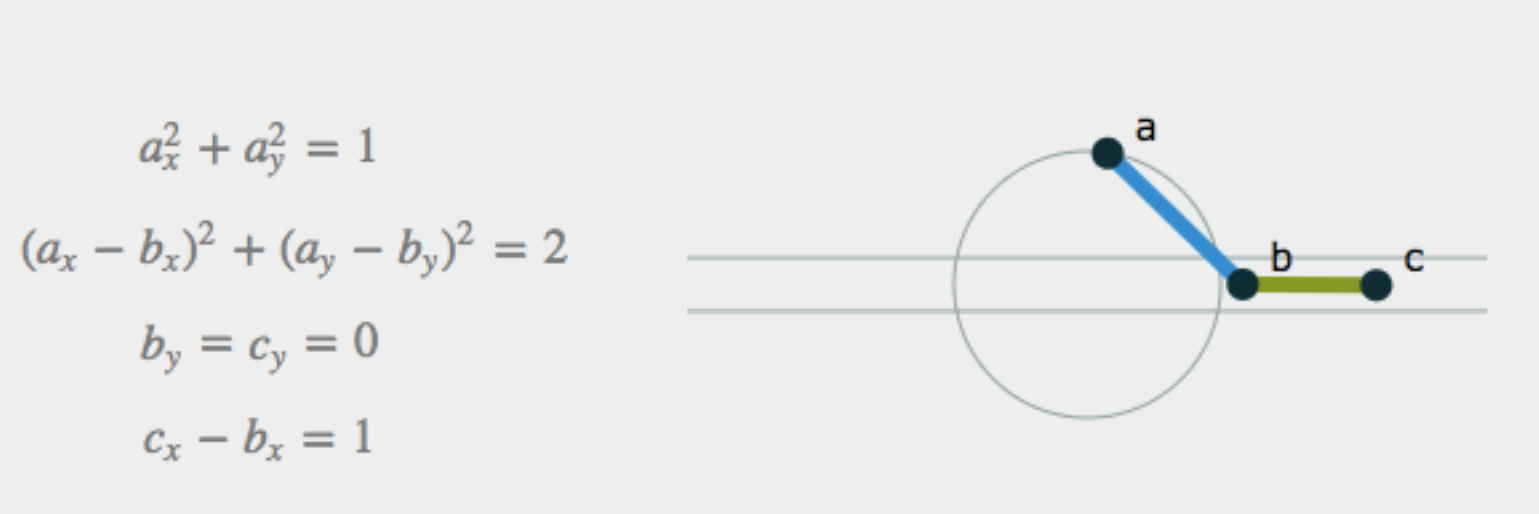
\includegraphics[width=\linewidth]{constraints.jpg}
  \caption{Parametric constraints represented as equations and inequalities; adapted from Ref. \cite{keeter}. }
  \label{fig:constraints}
\end{figure}

The interface allows the user to freely click-and-drag points around the canvas, which creates the problem of satisfying all the constraints in real-time. To tackle this problem, we found Cassowary.js \cite{cassowary}, a JavaScript library that implements a version of the simplex algorithm, which was created to solve {\it linear programming} problems.  A linear program consists of $n$ variables on which we have a linear objective function and a set of linear constraints. For example, the following is a linear program on $n=4$ variables.
\[\text{Minimize } C = x_1 + 3x_2 - 2x_4 \text{ subject to: }\]
\[x_1 + x_2 \geq 4,\]
\[x_3 - 4x_4 + x_2 = 42, \text{ and}\]
\[4x_1 + x_3 - x_2 \leq 2.\]

Therefore, we can formulate our geometric constraints as a linear program where each $x$ and $y$ value of every point in every shape is a variable and each geometric constraint is transformed into (possibly multiple) linear constraints. In addition to solving simple linear programs, Cassowary.js also allows us to specify non-required constraints of varying {\it strength}. For example, we can specify that we would like a particular point to stay where it is unless absolutely necessary. Because of this, we do not need to explicitly define an objective function for our linear program.

Some geometric constraints are easily transformed into linear (in)equalities, but others are not. For example, to constrain a line to be horizontal is easy, as we simply specify that the $x$ coordinates of its endpoints must be equal, but constraining a line to be a fixed length is much more difficult. Our solution was to cleverly reform and approximate many geometric constraints using more than one linear equation or inequality.

Below are the geometric constraints we implemented, along with a description of how they were implemented. 

\begin{itemize}
\item {\bf Fixed:} Constrains a point to stay in the same location. Implemented by setting the $x$- and $y$-coordinates to be constants.
\item {\bf Coincident:} Constrains two points to lie in the same location. Implemented by setting the x-coordinates to be equal and the y-coordinates to be equal.
\item {\bf Horizontal:} Constrains a line to be horizontal. Implemented by setting the x-coordinates of the two endpoints to be equal.
\item {\bf Vertical:} Constrains a line to be vertical. Implemented by setting the y-coordinates of the two endpoints to be equal.
\item {\bf Parallel:} Constrains two lines to be parallel. This constraint is more difficult to implement, as there is no way to represent it with linear equations. However, we can implement a fixed-slope constraint using linear equations by fixing the ratio between the difference of the $x$- and $y$- coordinates. So, when this constraint is initially set, we constrain both lines to have a fixed slope, and whenever an endpoint is moved, we programmatically update the slope of the constraint.
\item {\bf Perpendicular:} Constrains two lines to be perpendicular. This constraint is implemented exactly the same as the parallel constraint, except for setting both lines to have the same slope, one is set to have the negative reciprocal slope of the other and is updated programmatically in a similar way.
\item {\bf Length:} Constrains a line to be a fixed length. This was the most difficult constraint to implement, as the distance equation is very nonlinear, so instead we must approximate it with many linear inequalities. The {\it Manhattan distance} is defined as the sum of the absolute differences between the $x$- and $y$-coordinates of two points. So, we can estimate a Euclidean distance constraint with multiple Manhattan distance constraints in the following way. If we constrain a point to be within a fixed Manhattan distance of another point, the it will lie within a diamond centered at that point. Then, using linear equations, we can transform our coordinate system by a fixed angle and set another Manhattan distance distance constraint. This constraint will have the diamond rotated by that fixed angle. Enough of these constraints will approximate a circle. However, this only constrains two points to be {\it within} a fixed distance, so we must create minimum Manhattan distance constraints in a similar way. All of these together allows us to constrain the two endpoints of a line to a fixed distance from each other. This process is illustrated in Figures \ref{dist1} through \ref{dist3}.
\end{itemize}

\begin{figure}[H]
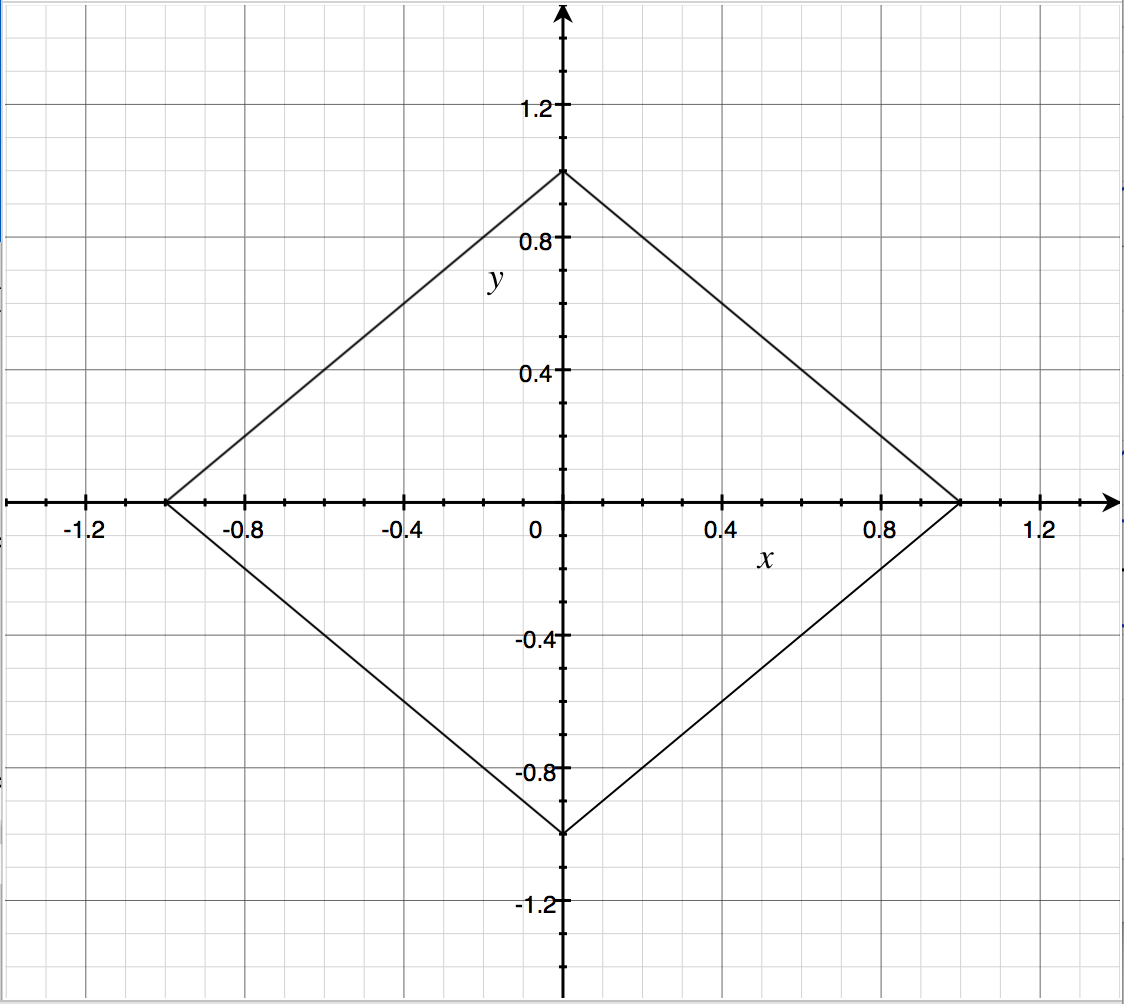
\includegraphics[width=\linewidth]{dist1.png}
\caption{The region constrained by $|x| + |y| \leq 1$.}
\label{dist1}
\end{figure}

\begin{figure}[H]
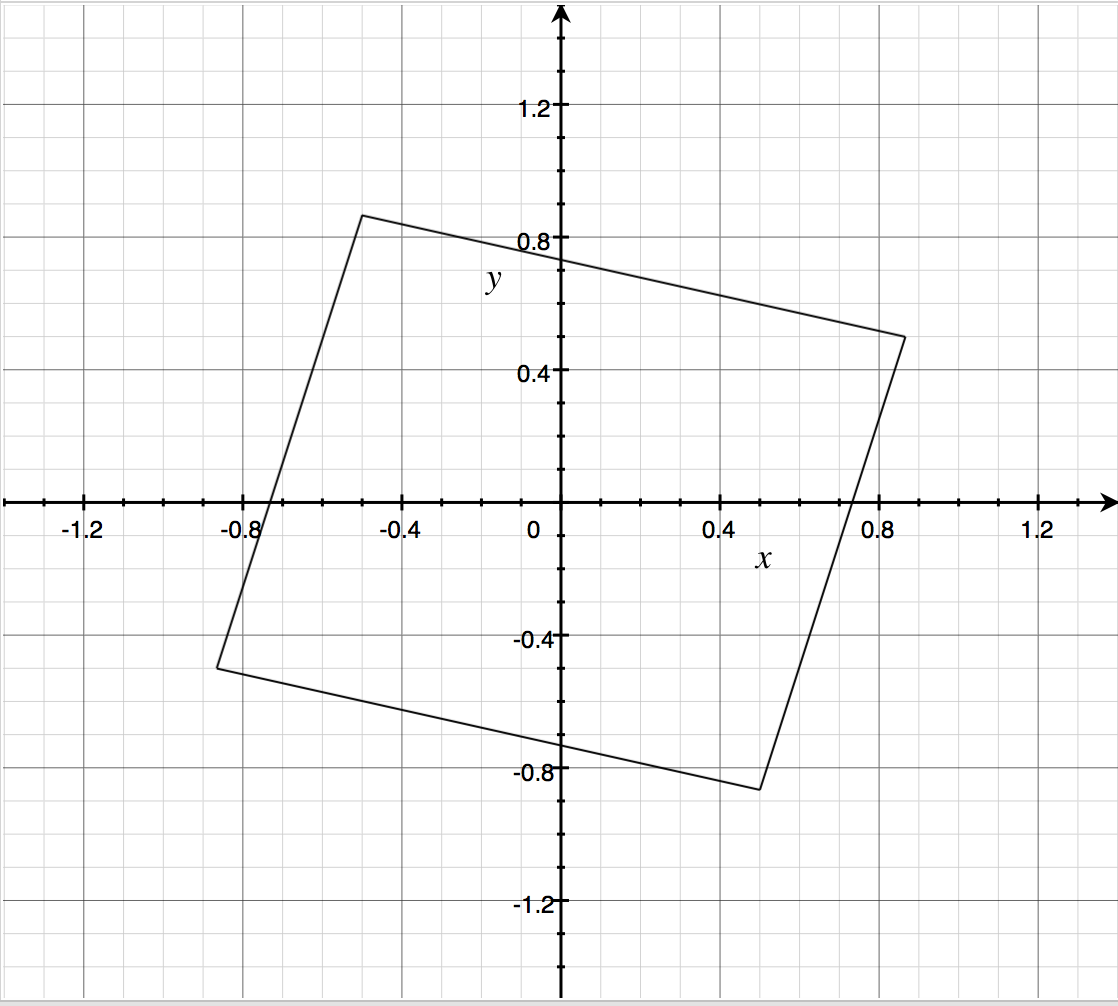
\includegraphics[width=\linewidth]{dist2.png}
\caption{The region constrained by $|x'| + |y'| \leq 1$ where $x'$ and $y'$ are the coordinates of the point in the coordinate system rotated by 30$^\circ$.}
\label{dist2}
\end{figure}

\begin{figure}[H] 
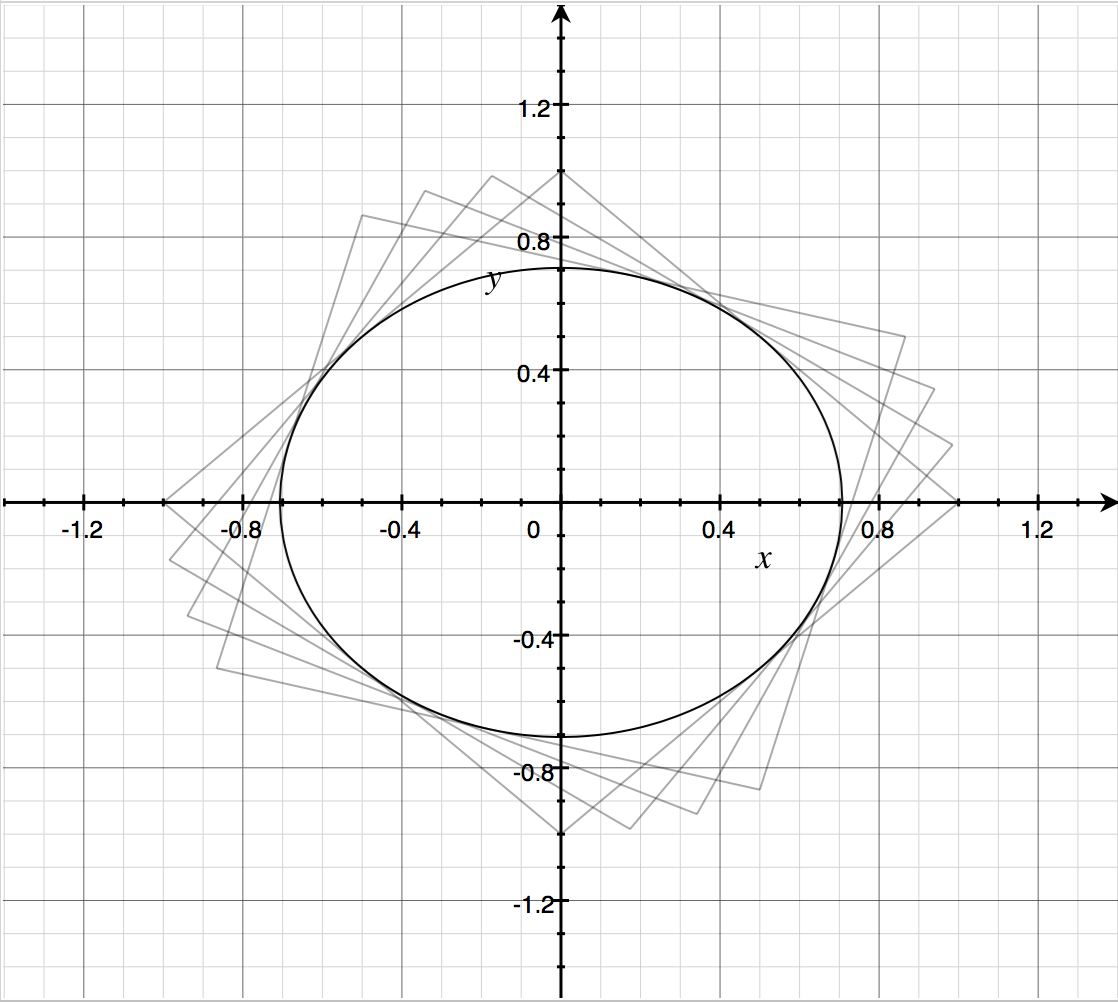
\includegraphics[width=\linewidth]{dist3.png}
\caption{With enough of these regions, we approximate the circle of radius $\frac{\sqrt{2}}{2}$ about the origin.}
\label{dist3}
\end{figure}

\subsection*{Direct Transformations}

2to3D implements three direct transformations: move, scale, and rotate. These tools allow users to specify geometry which will not be modified by the geometric constraint solver while being transformed. This is done by creating a new set of points at the respective locations of the points that compose the selected shapes. These points are then mapped to new locations through a $x-$/$y-$ translation function, a rotation function, or a scale function. Finally the original shapes are deleted leaving only the newly transformed shapes.

The transformation function translates all points by the displacement of the mouse from the initial selection point. The rotation function rotates all points around a centroid (pivot point) by the angle formed by the line which passes through the initial selection point and the pivot and the line which passes through the current cursor point and the pivot. The scale function works by forming a circle with radius equal to the distance between the initial selection point and the pivot. As the cursor is dragged farther from the pivot outside the circle the selected shapes are scaled up. As the cursor is dragged closer to the pivot inside the circle the selected shapes are scaled down.

\subsection*{Link to GitHub Repository}

The full implementation can be found at \newline \underline{\url{https://github.com/leomcelroy/2to3D}}.

\subsection*{Link to Video Demo}

A video demoing the capabilities of 2to3D can be found at \newline \underline{\url{https://www.youtube.com/watch?v=QDdJkAFzwLU}}.


\section{Results}

\subsection*{Other Capabilities}

We produced a highly accessible CAD program suitable for laser cutting. The accessibility of 2to3D can be attributed to the fact that the program runs entirely in the browser (thus requiring no additional software beyond a modern browser), and that the program strips away all non-essential drawing features and all 3D modeling features. Currently 2to3D only supports the creation of drawings intended for translation into cutting paths. Figure~\ref{fig:usingProgram} depicts a full digital fabrication workflow using 2to3D. The figure depicts the design of a press-fit box. The laser cutter available for use utilized CorelDRAW for CAM so the drawing was exported from 2to3D as a SVG and imported to CorelDRAW for printing.

\begin{figure}[H]
  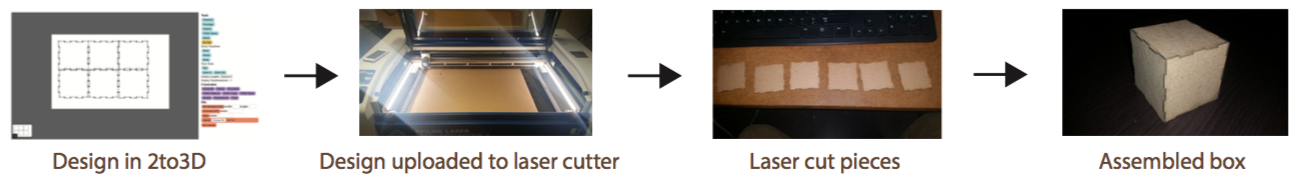
\includegraphics[width=\linewidth]{usingProgram.jpg}
  \caption{Full digital fabrication workflow using 2to3D. The laser cutter we had access to used CorelDraw for CAM so the drawing was created in 2to3D and imported to CorelDraw just for printing.}
  \label{fig:usingProgram}
\end{figure}

2to3D has a simple design that displays all tools to the user without being overwhelming. This design inspired by ``lean-operating practices" also immediately and constantly conveys program state information by highlighting the current tool and changing the cursor style. Figures \ref{fig:screenshot} and \ref{fig:screenshot2} are screenshots of the program.

\begin{figure}[H]
  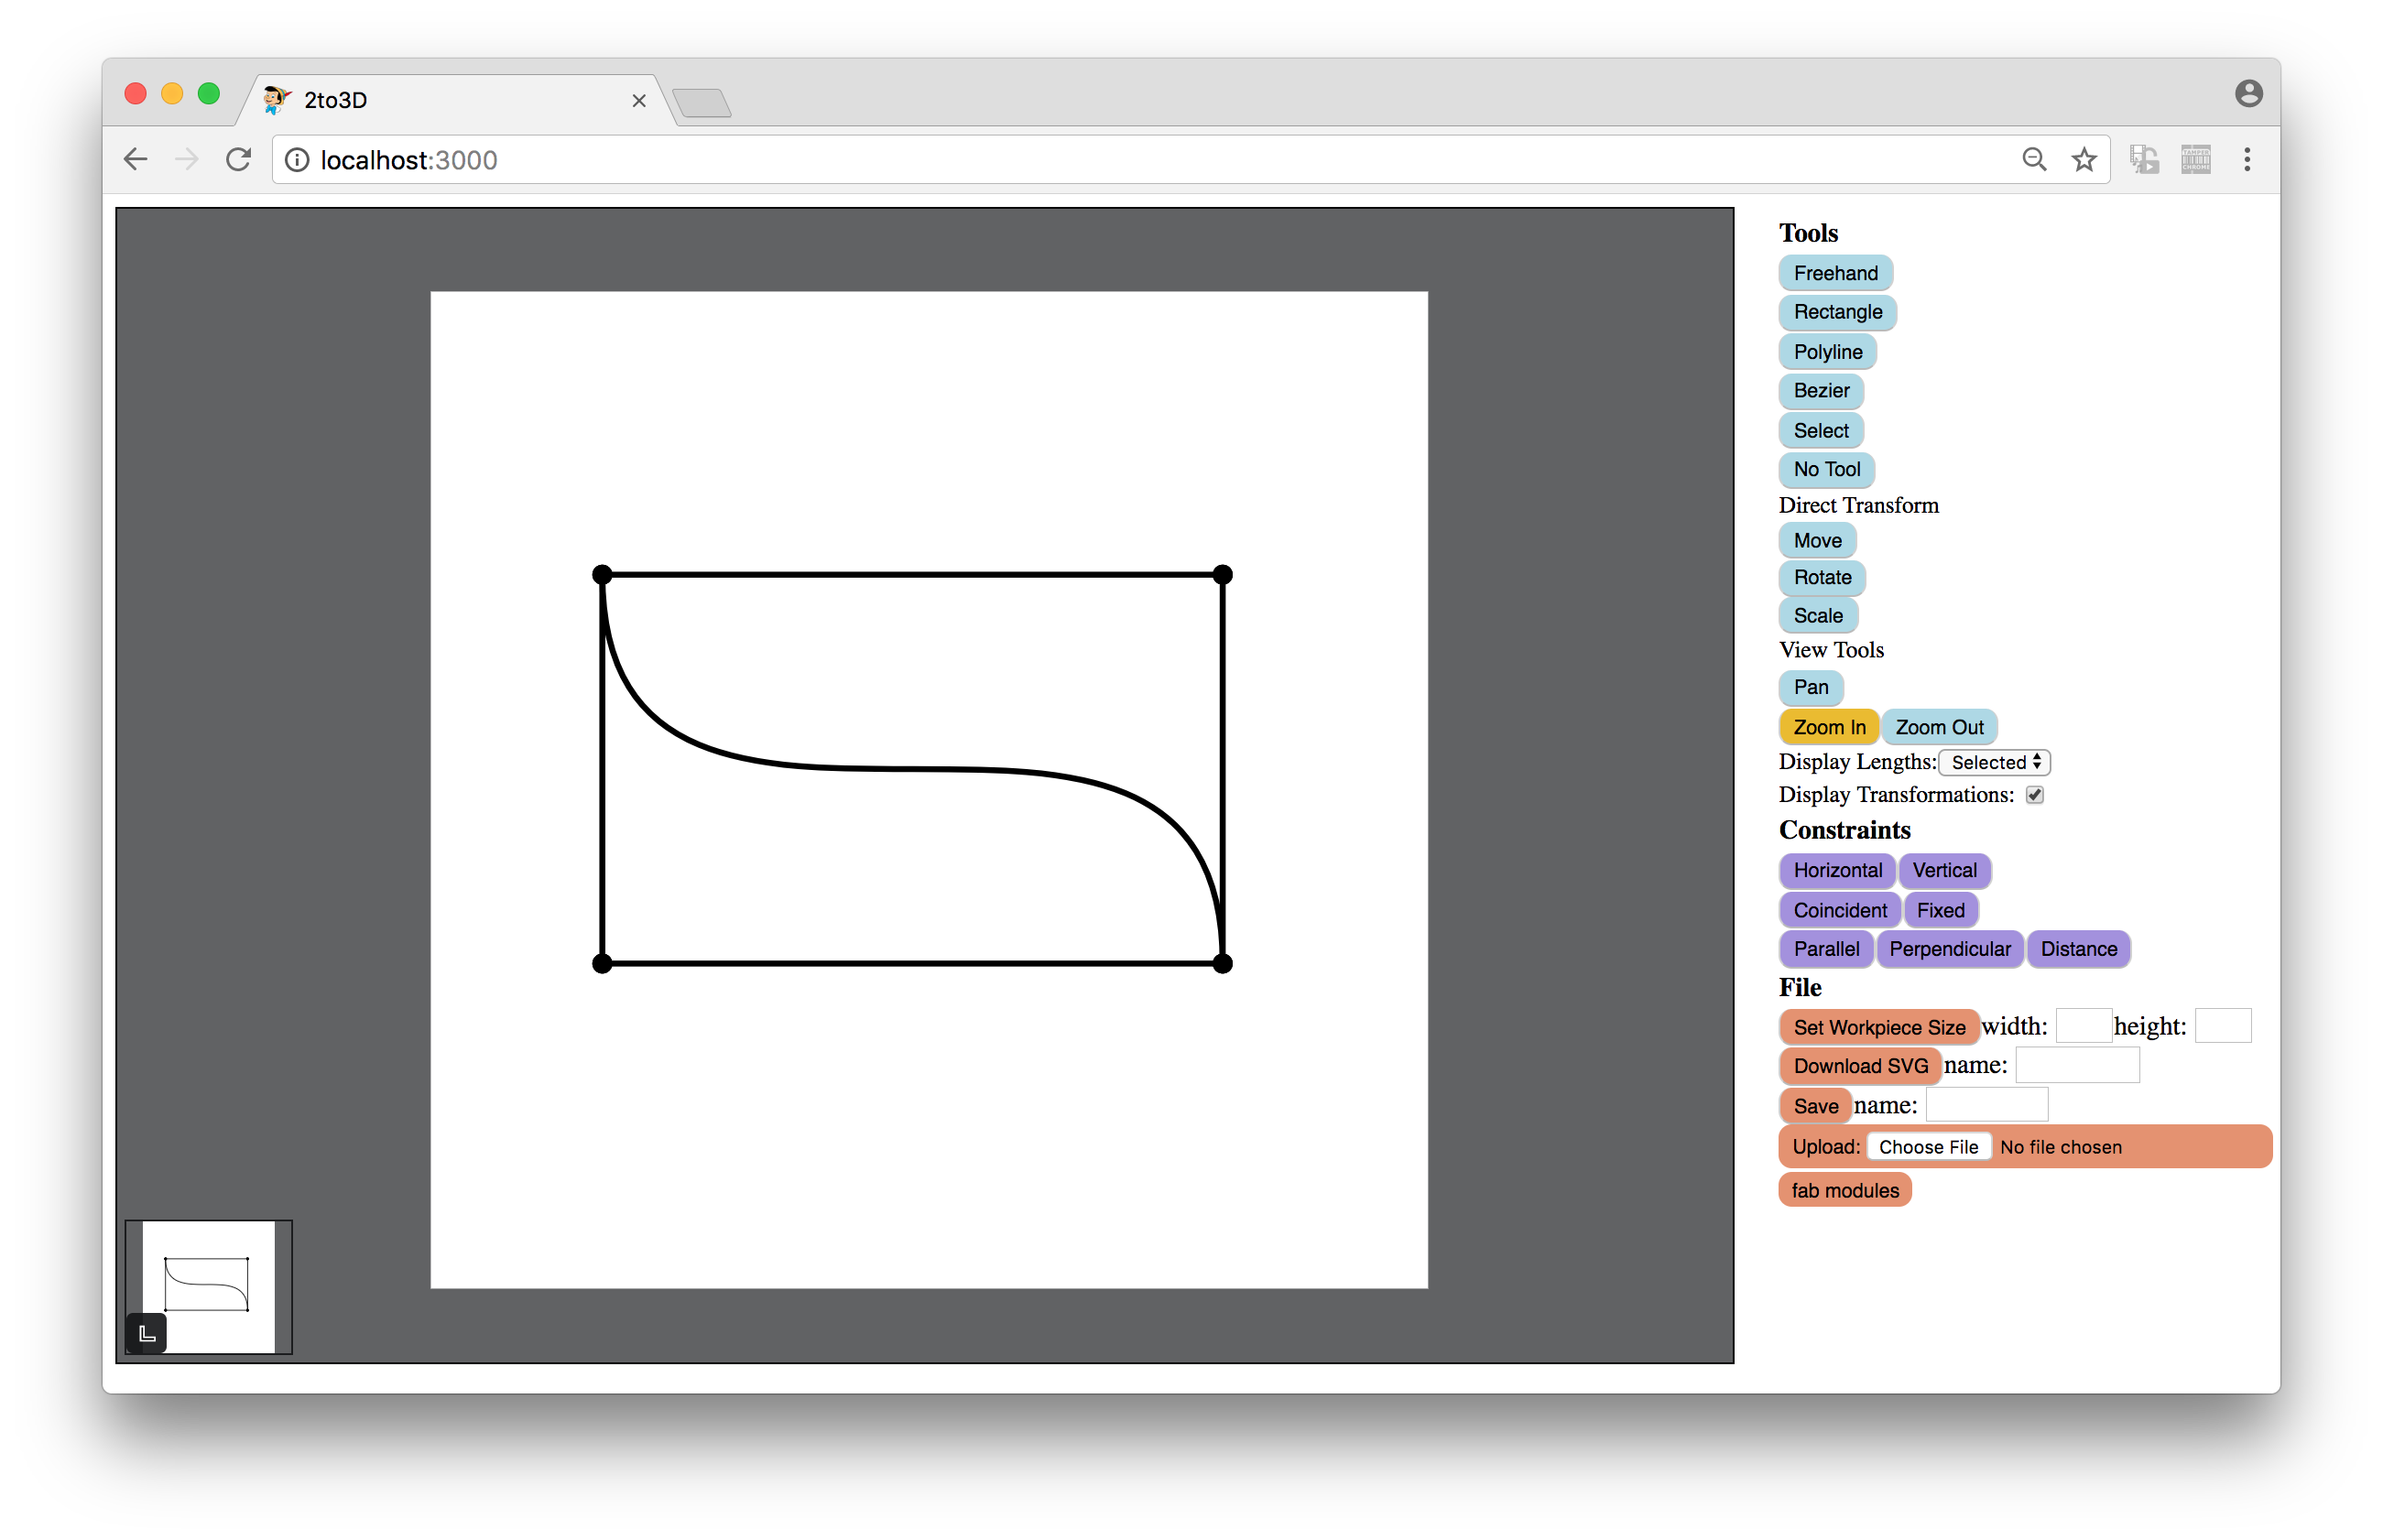
\includegraphics[width=\linewidth]{screenshot.png}
  \caption{Screenshot of 2to3D program depicting example bezier and rectangle.}
  \label{fig:screenshot}
\end{figure}

\begin{figure}[H]
  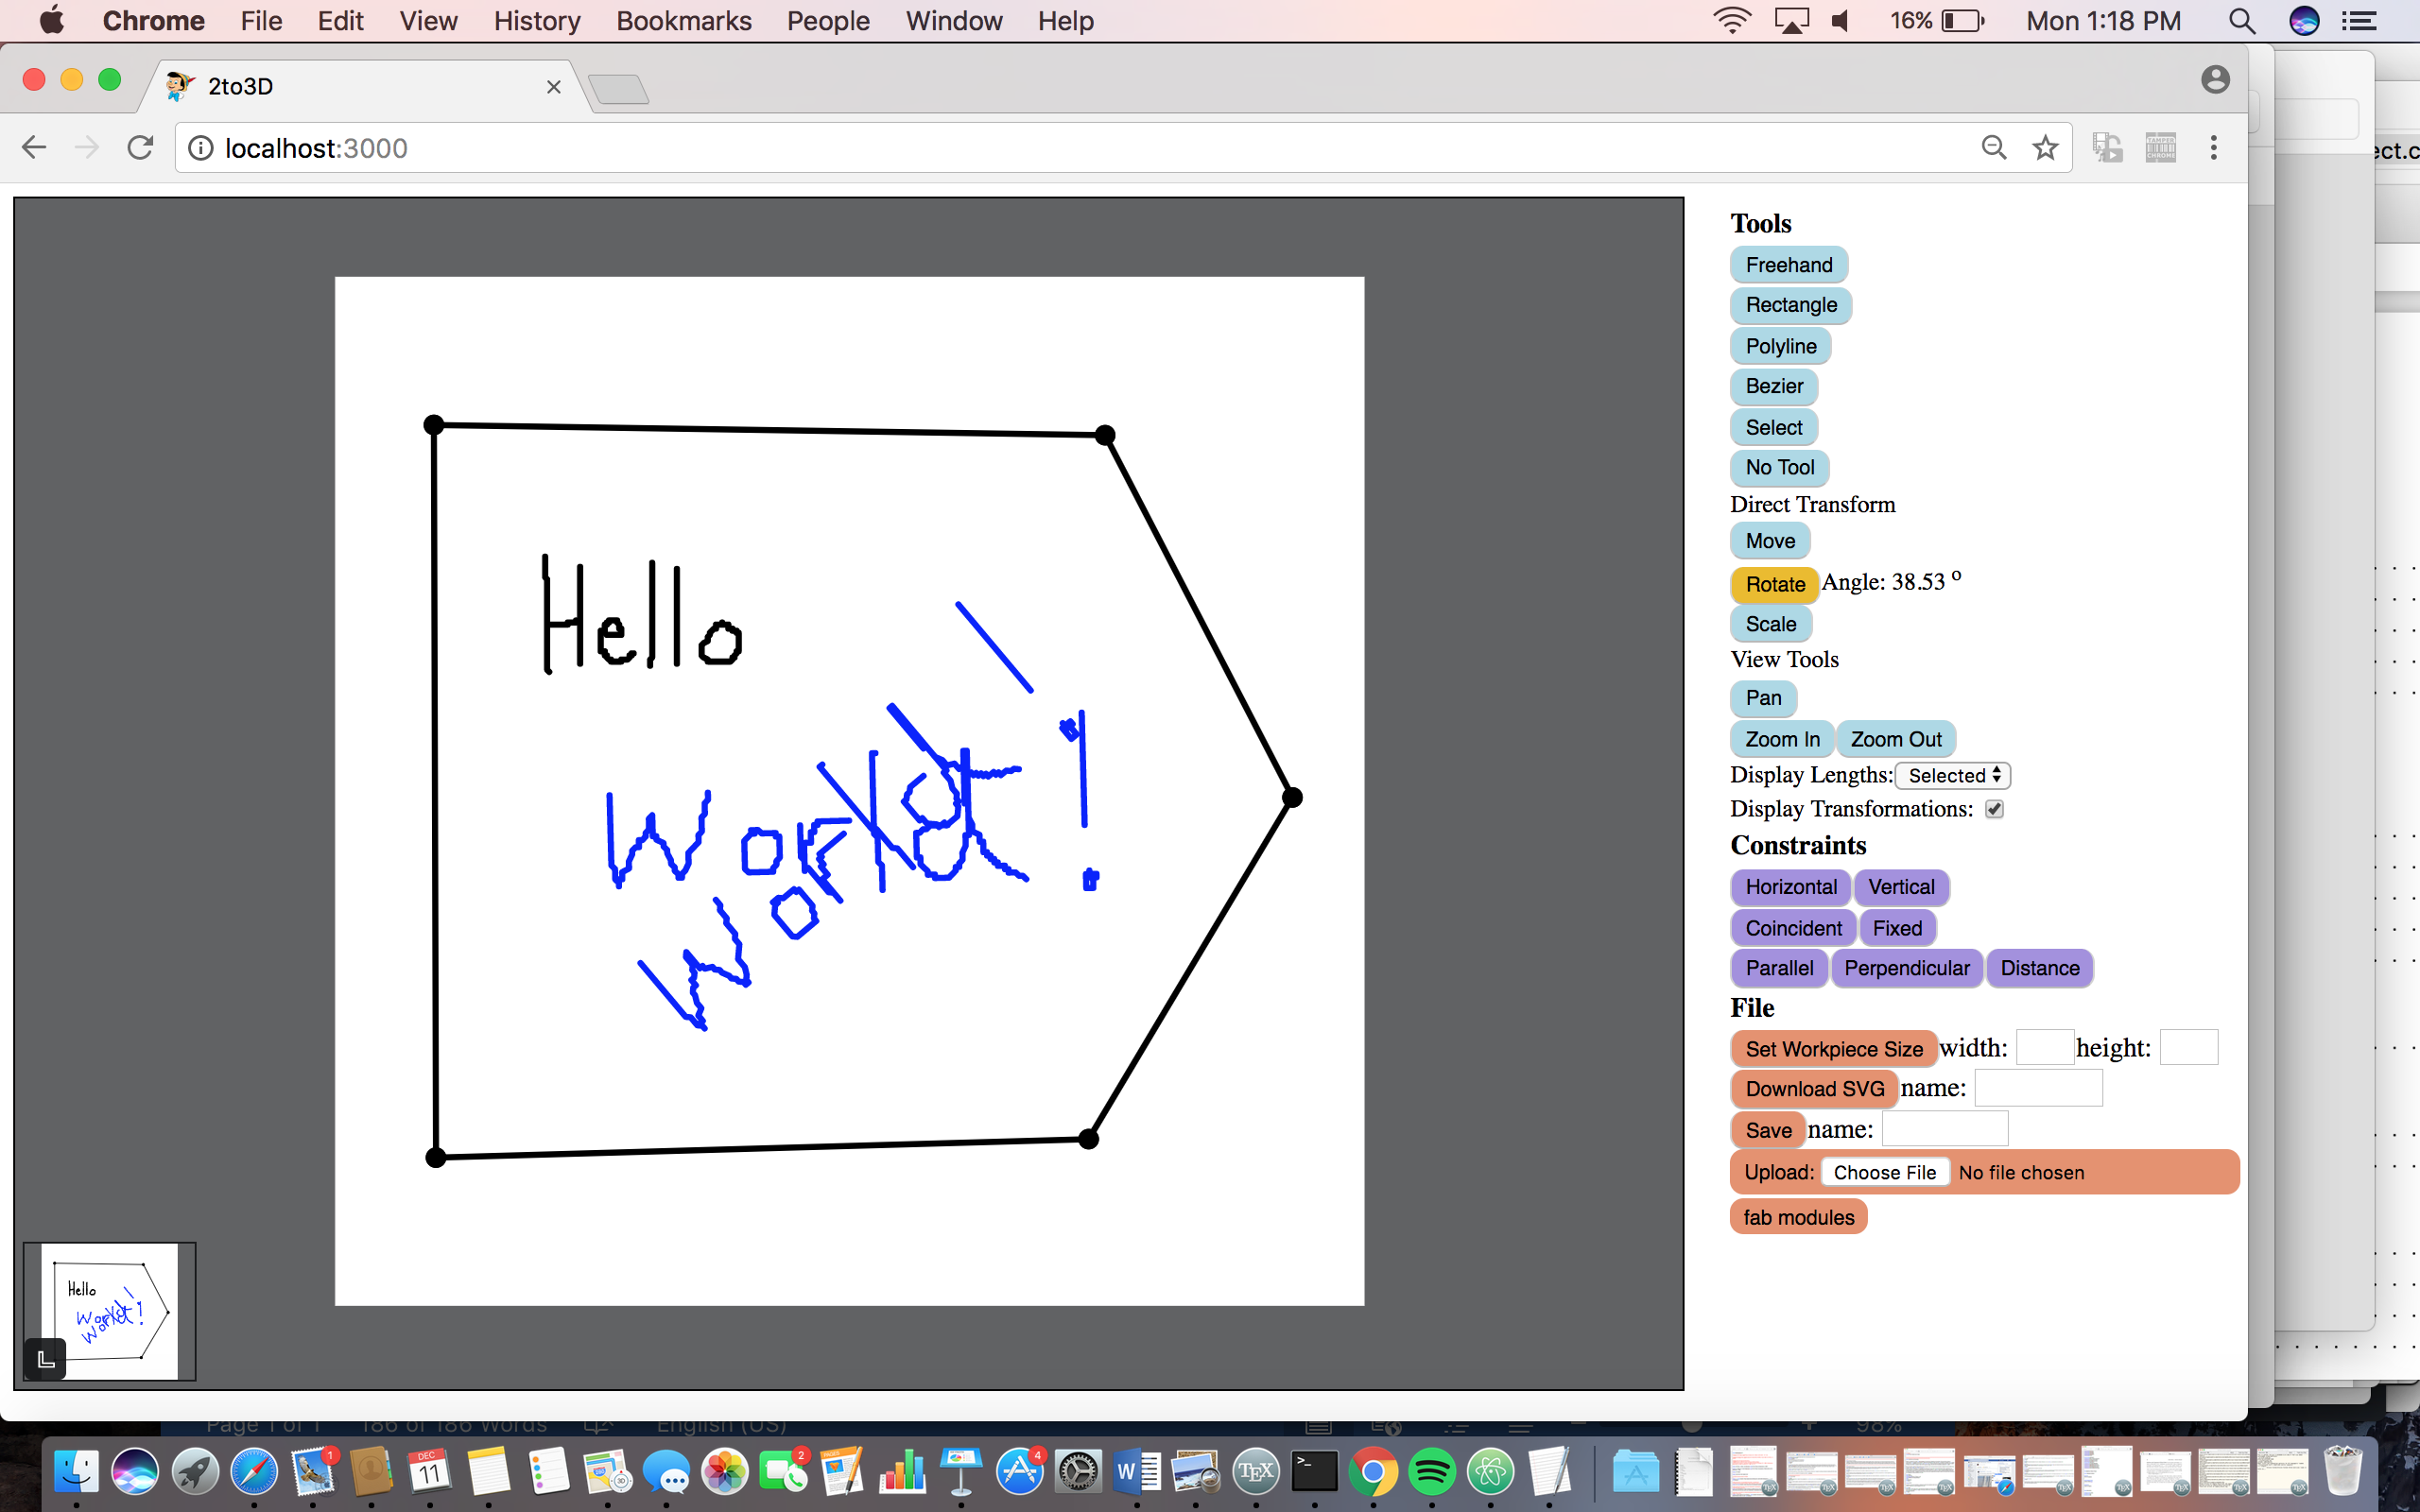
\includegraphics[width=\linewidth]{screenshot2.png}
  \caption{Screenshot of 2to3D program depicting rotation tool in action. Note the angle on display next to the highlights tool in the right toolbox.}
  \label{fig:screenshot2}
\end{figure}

2to3D supports three shape primitives (line, bezier and freehand) which can be used to create more complex shapes. The program supports both linear and non-linear constraints but linear constraints are far more robust. The program also supports direct transformations - rotations, moves, and scales - that break constraints of transformed objects. This allows the user to make direct edits to drawing geometry that will exactly reflect user's intention. In addition to these three aspects which were detailed in Section 4, 2to3D also supports a myriad of other features. The drawing area allows zooming in/out and panning and the workpiece size is adjustable which facilitates creation of designs on any scale. SVG exports draw dimensions from workpiece size which simplifies the CAM process if the user decides to match drawing dimensions to laser cutter bed size. Hotkeys support swift and smooth workflows and copy and paste capabilities allow users to quickly create redundant geometry. Geometry can also be deleted to correct errors. A save and upload feature also allows users to continue work on unfinished projects or to share designs with others. A full list of features can be found in Table~\ref{tab:capabilities}.

\begin{table}[H]
\centering
\caption{Capabilities of 2to3D.}
\label{tab:capabilities}
\begin{tabular}{|l|l|l|l|}
\hline
\multicolumn{2}{|l|}{{\ul \textbf{Drawing}}}                                                                                                                                                        & \multicolumn{2}{l|}{{\ul \textbf{Navigation}}}                                                                                                                                               \\
\multicolumn{2}{|l|}{\begin{tabular}[c]{@{}l@{}}Freehand\\ Rectangle\\ Polyline\\ Bezier\end{tabular}}                                                                                              & \multicolumn{2}{l|}{\begin{tabular}[c]{@{}l@{}}Pan\\ Zoom in/out\end{tabular}}                                                                                                               \\ \hline
\multicolumn{2}{|l|}{{\ul \textbf{Direct Transformations}}}                                                                                                                                         & \multicolumn{2}{l|}{{\ul \textbf{Display Options}}}                                                                                                                                          \\
\multicolumn{2}{|l|}{\begin{tabular}[c]{@{}l@{}}Move\\ Rotate\\ Scale\end{tabular}}                                                                                                                 & \multicolumn{2}{l|}{\begin{tabular}[c]{@{}l@{}}Lengths\\ Transformation values\end{tabular}}                                                                                                 \\ \hline
\multicolumn{2}{|l|}{{\ul \textbf{Constraints}}}                                                                                                                                                    & \multicolumn{2}{l|}{{\ul \textbf{Other}}}                                                                                                                                                    \\
\multicolumn{2}{|l|}{\begin{tabular}[c]{@{}l@{}}Horizontal (line)\\ Vertical (line)\\ Coincident (points)\\ Fixed (points)\\ Parallel (lines)\\ Perpendicular (lines)\\ Length (line)\end{tabular}} & \multicolumn{2}{l|}{\begin{tabular}[c]{@{}l@{}}Click and drag points\\ Download SVG\\ Save drawing\\ Upload drawing\\ Copy/Paste\\ Delete\\ Hotkeys\\ Workpiece size adjustable\end{tabular}} \\ \hline
\end{tabular}
\end{table}

\subsection*{Link to Video Demo and Program}
A demonstration of the program's features can be found at: \newline \underline{\url{https://www.youtube.com/watch?v=QDdJkAFzwLU}}. \newline

The program itself can be accessed while on Middlebury College's network at: \newline \underline{\url{basin.cs.middlebury.edu:3002}}.

\section{Discussion}

%This section should begin with a brief summary of your results. Next, provide a
%more detailed synopsis of your results: What new knowledge do they offer? What
%lessons did you learn? What is the main take-away message of your work?
%Finally, you should provide a brief critique of your own work: Point out the
%specific attributes that you feel are extremely positive and note any
%weaknesses or limitations. Discuss how your project could be improved. You can
%also discuss possible extensions of your work. This section should be
%approximately 1 page in length.

We accomplished our main goal of creating a parametric web-based vector drawing program, but as with all software engineering, the work is never done. Future work would include the following goals:

- Build out shape primitives to include circles and arcs, as well as associated constraints (such as tangent).

- Improve the program?s state-handling to enhance user experience. This could involve introducing atomic operations which would allow tracking of a file?s timeline.

- Create a JavaScript library that can efficiently solve systems of nonlinear equations using gradient descent.

- Integrate 2to3D with existing open-source web-based CAM software such as MIT?s Center for Bits and Atoms? ?fab modules.?


%ACKNOWLEDGMENTS are optional
\section{Acknowledgments}

This section is optional; it is a location for you to acknowledge grants,
assistance, etc. For example, this report template was adapted from Prof.
Christman.



\bibliographystyle{abbrv}
\bibliography{references}  % references.bib is the name of the BibTex file

\end{document}
